%%%%%%%%%%%%%%
%% Run LaTeX on this file several times to get Table of Contents,
%% cross-references, and citations.

%% If you have font problems, you may edit the w-bookps.sty file
%% to customize the font names to match those on your system.

%% w-bksamp.tex. Current Version: Feb 16, 2012
%%%%%%%%%%%%%%%%%%%%%%%%%%%%%%%%%%%%%%%%%%%%%%%%%%%%%%%%%%%%%%%%
%
%  Sample file for
%  Wiley Book Style, Design No.: SD 001B, 7x10
%  Wiley Book Style, Design No.: SD 004B, 6x9
%
%
%  Prepared by Amy Hendrickson, TeXnology Inc.
%  http://www.texnology.com
%%%%%%%%%%%%%%%%%%%%%%%%%%%%%%%%%%%%%%%%%%%%%%%%%%%%%%%%%%%%%%%%

%%%%%%%%%%%%%
% 7x10
%\documentclass{wileySev}

% 6x9
\documentclass{wileySix}

\usepackage{graphicx}
\usepackage{listings}

\usepackage{color}

\definecolor{codegreen}{rgb}{0,0.6,0}
\definecolor{codegray}{rgb}{0.5,0.5,0.5}
\definecolor{codepurple}{rgb}{0.58,0,0.82}
\definecolor{backcolour}{rgb}{0.95,0.95,0.92}

\lstdefinestyle{mystyle}{
    backgroundcolor=\color{backcolour},
    commentstyle=\color{codegreen},
    keywordstyle=\color{magenta},
    numberstyle=\tiny\color{codegray},
    stringstyle=\color{codepurple},
    basicstyle=\footnotesize,
    breakatwhitespace=false,
    breaklines=true,
    captionpos=b,
    keepspaces=true,
    numbers=left,
    numbersep=5pt,
    showspaces=false,
    showstringspaces=false,
    showtabs=false,
    tabsize=2,
    language=sh
}

\lstset{style=mystyle}

%%%%%%%
%% for times math: However, this package disables bold math (!)
%% \mathbf{x} will still work, but you will not have bold math
%% in section heads or chapter titles. If you don't use math
%% in those environments, mathptmx might be a good choice.

% \usepackage{mathptmx}

% For PostScript text
\usepackage{w-bookps}

%%%%%%%%%%%%%%%%%%%%%%%%%%%%%%%%%%%%%%%%%%%%%%%%%%%%%%%%%%%%%%%%
%% Other packages you might want to use:

% for chapter bibliography made with BibTeX
% \usepackage{chapterbib}

% for multiple indices
% \usepackage{multind}

% for answers to problems
% \usepackage{answers}

%%%%%%%%%%%%%%%%%%%%%%%%%%%%%%
%% Change options here if you want:
%%
%% How many levels of section head would you like numbered?
%% 0= no section numbers, 1= section, 2= subsection, 3= subsubsection
%%==>>
\setcounter{secnumdepth}{3}

%% How many levels of section head would you like to appear in the
%% Table of Contents?
%% 0= chapter titles, 1= section titles, 2= subsection titles,
%% 3= subsubsection titles.
%%==>>
\setcounter{tocdepth}{2}

%% Cropmarks? good for final page makeup
%% \docropmarks

%%%%%%%%%%%%%%%%%%%%%%%%%%%%%%
%
% DRAFT
%
% Uncomment to get double spacing between lines, current date and time
% printed at bottom of page.
% \draft
% (If you want to keep tables from becoming double spaced also uncomment
% this):
% \renewcommand{\arraystretch}{0.6}
%%%%%%%%%%%%%%%%%%%%%%%%%%%%%%

%%%%%%% Demo of section head containing sample macro:
%% To get a macro to expand correctly in a section head, with upper and
%% lower case math, put the definition and set the box
%% before \begin{document}, so that when it appears in the
%% table of contents it will also work:

\newcommand{\VT}[1]{\ensuremath{{V_{T#1}}}}

%% use a box to expand the macro before we put it into the section head:

\newbox\sectsavebox
\setbox\sectsavebox=\hbox{\boldmath\VT{xyz}}

%%%%%%%%%%%%%%%%% End Demo


\begin{document}


\booktitle{Deep Learning A-Z : Hands-On Artificial Neural Networks}
%\subtitle{Dalam 24 Jam}

\authors{Rolly M. Awangga\\
\affil{Informatics Research Center}
%Floyd J. Fowler, Jr.\\
%\affil{University of New Mexico}
}

\offprintinfo{Learn to create Deep Learning Algorithms in Python from two Machine Learning \& Data Science experts. Templates included.}{Rolly M. Awangga}

%% Can use \\ if title, and edition are too wide, ie,
%% \offprintinfo{Survey Methodology,\\ Second Edition}{Robert M. Groves}

%%%%%%%%%%%%%%%%%%%%%%%%%%%%%%
%%
\halftitlepage

\titlepage


\begin{copyrightpage}{2019}
%Survey Methodology / Robert M. Groves . . . [et al.].
%\       p. cm.---(Wiley series in survey methodology)
%\    ``Wiley-Interscience."
%\    Includes bibliographical references and index.
%\    ISBN 0-471-48348-6 (pbk.)
%\    1. Surveys---Methodology.  2. Social 
%\  sciences---Research---Statistical methods.  I. Groves, Robert M.  II. %
%Series.\\
%
%HA31.2.S873 2007
%001.4'33---dc22                                             2004044064
\end{copyrightpage}

\dedication{`Jika Kamu tidak dapat menahan lelahnya belajar,
Maka kamu harus sanggup menahan perihnya Kebodohan.'
~Imam Syafi'i~}

\begin{contributors}
\name{Rolly Maulana Awangga,} Informatics Research Center., Politeknik Pos Indonesia, Bandung,
Indonesia



\end{contributors}

\contentsinbrief
\tableofcontents
\listoffigures
\listoftables
\lstlistoflistings


\begin{foreword}
Sepatah kata dari Kaprodi, Kabag Kemahasiswaan dan Mahasiswa
\end{foreword}

\begin{preface}
Buku ini diciptakan bagi yang awam dengan git sekalipun.

\prefaceauthor{R. M. Awangga}
\where{Bandung, Jawa Barat\\
Februari, 2019}
\end{preface}


\begin{acknowledgments}
Terima kasih atas semua masukan dari para mahasiswa agar bisa membuat buku ini 
lebih baik dan lebih mudah dimengerti.

Terima kasih ini juga ditujukan khusus untuk team IRC yang 
telah fokus untuk belajar dan memahami bagaimana buku ini mendampingi proses 
Intership.
\authorinitials{R. M. A.}
\end{acknowledgments}

\begin{acronyms}
\acro{ACGIH}{American Conference of Governmental Industrial Hygienists}
\acro{AEC}{Atomic Energy Commission}
\acro{OSHA}{Occupational Health and Safety Commission}
\acro{SAMA}{Scientific Apparatus Makers Association}
\end{acronyms}

\begin{glossary}
\term{git}Merupakan manajemen sumber kode yang dibuat oleh linus torvald.

\term{bash}Merupakan bahasa sistem operasi berbasiskan *NIX.

\term{linux}Sistem operasi berbasis sumber kode terbuka yang dibuat oleh Linus Torvald
\end{glossary}

\begin{symbols}
\term{A}Amplitude

\term{\hbox{\&}}Propositional logic symbol 

\term{a}Filter Coefficient

\bigskip

\term{\mathcal{B}}Number of Beats
\end{symbols}

\begin{introduction}

%% optional, but if you want to list author:

\introauthor{Rolly Maulana Awangga, S.T., M.T.}
{Informatics Research Center\\
Bandung, Jawa Barat, Indonesia}

Pada era disruptif  \index{disruptif}\index{disruptif!modern} 
saat ini. git merupakan sebuah kebutuhan dalam sebuah organisasi pengembangan perangkat lunak.
Buku ini diharapkan bisa menjadi penghantar para programmer, analis, IT Operation dan Project Manajer.
Dalam melakukan implementasi git pada diri dan organisasinya.

Rumusnya cuman sebagai contoh aja biar keren\cite{awangga2018sampeu}.

\begin{equation}
ABC {\cal DEF} \alpha\beta\Gamma\Delta\sum^{abc}_{def}
\end{equation}

\end{introduction}

%%%%%%%%%%%%%%%%%%Isi Buku_

\chapter{Pendahuluan}
\section{Latar Belakang}
\subsection{Sejarah Deep Learning}
Deep Learning mulai diperkenalkan di tahun 2006. Pada tahun 2006, Geoffrey Hinton (pada gambar \ref{labelgambar1} ) memperkenalkan salah satu varian jaringan saraf tiruan yang disebut deep belief nets, ide untuk men-train model jaringan saraf tiruan ini adalah dengan men-train dua layer kemudian tambahkan satu layer diatasnya, kemudian train hanya layer teratas dan begitu seterusnya. Dengan strategi ini dapat men-train model jaringan saraf tiruan dengan layer lebih banyak dari model-model sebelumnya. 

\begin{figure}[h!]
	\centering
	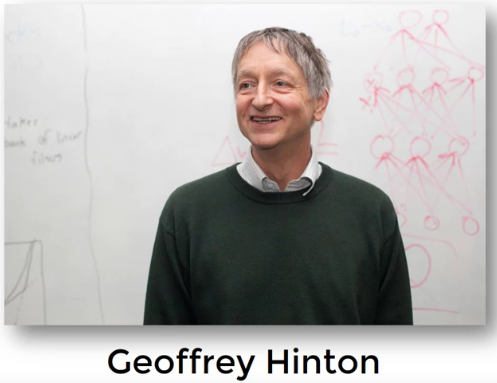
\includegraphics[scale=0.4]{figures/7.PNG}
	\caption{Gambar Geoffrey Hinton}
	\label{labelgambar1}
	\end{figure}

Setelah istilah deep learning populer, deep learning belum menjadi daya tarik yang besar bagi para peneliti karena jaringan saraf tiruan dengan banyak layer memiliki kompleksitas algoritma yang besar, sehingga membutuhkan komputer dengan spesifikasi tinggi, dan tidak efisien secara komputasi saat itu. Hingga pada tahun 2009 penggunaan GPU untuk deep learning diperkenalkan melalui paper yang berjudul Large-scale Deep Unsupervised Learning using Graphics Processors. Dengan menggunakan GPU jaringan saraf tiruan dapat berjalan lebih cepat dibanding dengan menggunakan CPU. Dengan tersedianya hardware yang memadai perkembangan deep learning mulai pesat, dan menghasilkan produk-produk yang dapat kita nikmati saat ini seperti pengenal wajah, self-driving car, pengenal suara, dan lain lain.


\subsection{Deep Learning}
Deep Learning (Pembelajaran Dalam) atau sering dikenal dengan istilah Pembelajaran Struktural Mendalam (Deep Structured Learning) atau Pembelajaran Hierarki (Hierarchical learning) adalah salah satu cabang dari ilmu pembelajaran mesin (Machine Learning) yang terdiri algoritma pemodelan abstraksi tingkat tinggi pada data menggunakan sekumpulan fungsi transformasi non-linear yang ditata berlapis-lapis dan mendalam.

Deep Learning adalah salah satu jenis algoritma jaringan saraf tiruan yang menggunakan metadata sebagai input dan mengolahnya menggunakan sejumlah lapisan tersembunyi (hidden layer) transformasi non linier dari data masukan untuk menghitung nilai output. Algortima pada Deep Learning memiliki fitur yang unik yaitu sebuah fitur yang mampu mengekstraksi secara otomatis. Hal ini berarti algoritma yang dimilikinya secara otomatis dapat menangkap fitur yang relevan sebagai keperluan dalam pemecahan suatu masalah.

\subsection{Artificial Neural Network}
Neural network adalah model yang terinspirasi oleh bagaimana neuron dalam otak manusia bekerja. Tiap neuron pada otak manusia saling berhubungan dan informasi mengalir dari setiap neuron tersebut. Neural Network sebenarnya mengadopsi dari kemampuan otak manusia yang mampu memberikan stimulasi/rangsangan, melakukan proses, dan memberikan output. Output diperoleh dari variasi stimulasi dan proses yang terjadi di dalam otak manusia. Kemampuan manusia dalam memproses informasi merupakan hasil kompleksitas proses di dalam otak. Misalnya, yang terjadi pada anak-anak, mereka mampu belajar untuk melakukan pengenalan meskipun mereka tidak mengetahui algoritma apa yang digunakan.







\chapter{Python}
\section{Perintah Navigasi}

\subsection{Installing Python And Anaconda}
\begin{enumerate}
  \item Download dan instal Python terbaru, versi 3.7.2
  \item Setelah selesai instal Python, download dan instal aplikasi Anaconda.
  \item Instal Anaconda dengan klik kanan aplikasi Anaconda.exe yang telah didownload tadi, kemudian Run as administrator.
      \begin{figure}[!ht]
	  \centering
	  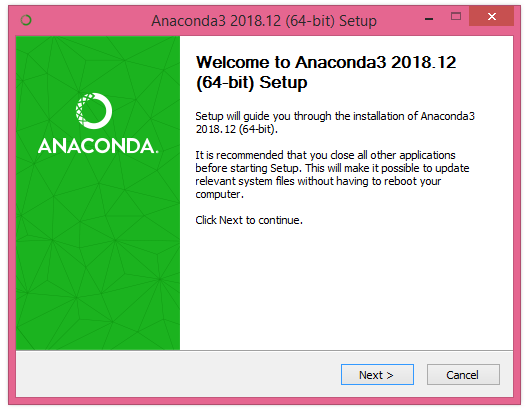
\includegraphics[scale=0.4]{figures/instal/1.PNG}
	  \caption{Instalasi Anaconda Proses 1}
	  \label{labelgambar2}
	  \end{figure}
  \item Kemudian pilih next (pada gambar \ref{labelgambar2}).
	 \begin{figure}[h]
	  \centering
	  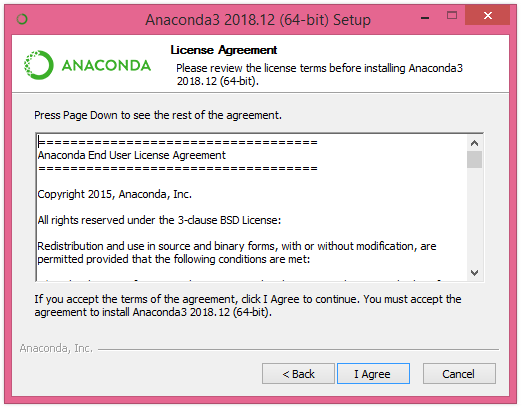
\includegraphics[scale=0.4]{figures/instal/2.PNG}
	  \caption{Instalasi Anaconda Proses 2}
	  \label{labelgambar3}
	  \end{figure}
  \item Kemudidan pilih I Agree (pada gambar \ref{labelgambar3}).
\begin{figure}[h!]
	  \centering
	  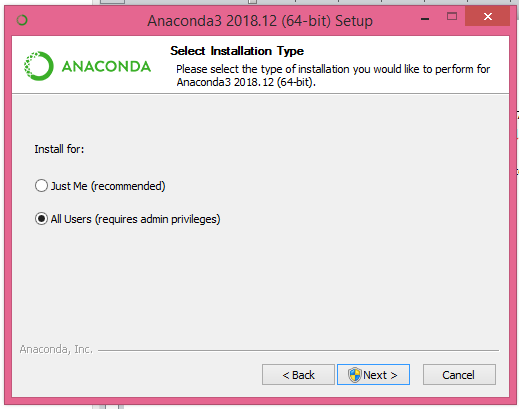
\includegraphics[scale=0.4]{figures/instal/3.PNG}
	  \caption{Instalasi Anaconda Proses 3}
	  \label{labelgambar4}
	  \end{figure}
  \item Pilih All User. kemudian klik Next (pada gambar \ref{labelgambar4}).
\begin{figure}[h!]
	  \centering
	  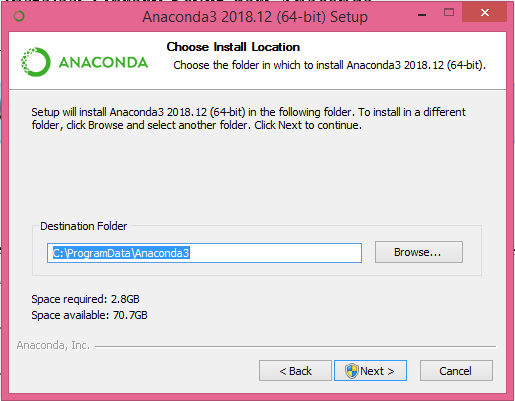
\includegraphics[scale=0.4]{figures/instal/4.PNG}
	  \caption{Instalasi Anaconda Proses 4}
	  \label{labelgambar5}
	  \end{figure}
  \item Tentukan directory instalasi. saya sarankan biarkan default saja. kemudian next (pada gambar \ref{labelgambar5}).
\begin{figure}[h!]
	  \centering
	  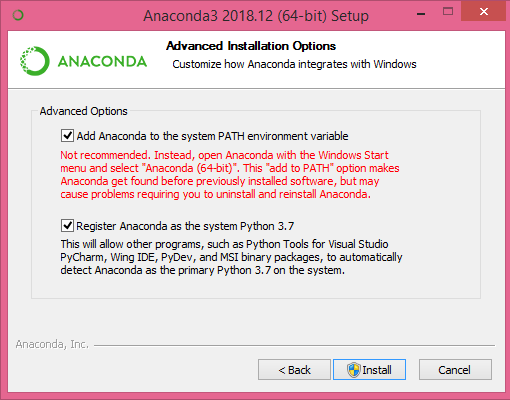
\includegraphics[scale=0.4]{figures/instal/5.PNG}
	  \caption{Instalasi Anaconda Proses 5}
	  \label{labelgambar6}
	  \end{figure}
  \item Kemudian centang pilihan Add Anaconda to the system PATH. kemudian pilih instal. Tunggu hingga proses instal selesai (pada gambar \ref{labelgambar6}).
  \item Setelah selesai klik next. Kemudian pilih install Microsoft VSCode. Tunggu hingga proses selesai (pada gambar \ref{labelgambar7})
      \begin{figure}[h!]
	  \centering
	  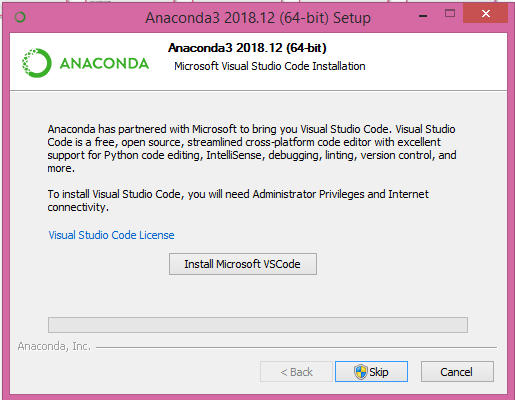
\includegraphics[scale=0.4]{figures/instal/8.PNG}
	  \caption{Instalasi Anaconda Proses 6}
	  \label{labelgambar7}
	  \end{figure}
  \item Setelah selesai, pilih Finish.

\end{enumerate}
\subsection{How to get the Dataset}
Untuk mempelajari tentang ANN, dibutuhkan dataset yang akan digunakan dan diolah untuk mengetahui proses kerja Artificial Neural Networks.
Data tersebut akan digunakan sebagai bahan untuk mempelajari ANNs.
Untuk mendapatkan dataset, prosesnya adalah sebagai berikut:
\begin{enumerate}
  \item Langkah pertama adalah dengan mengunjungi www.superdatascience.com/deep-learning.
  \item Untuk dataset ANNs, pilih dataset dan templates. Kemudian download template nya. (seperti pada gambar \ref{labelgambar8})
      \begin{figure}[h!]
	  \centering
	  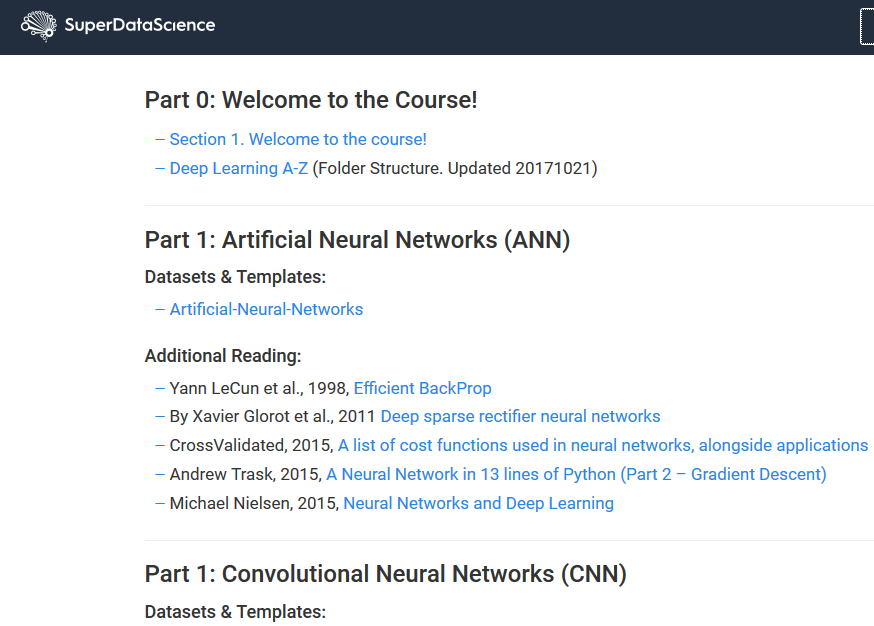
\includegraphics[scale=0.4]{figures/anns.PNG}
	  \caption{Tampilan Home SuperDataScience}
	  \label{labelgambar8}
	  \end{figure}
  \item Kemudian pilih Artificial-Neural-Networks.
  \item Dataset akan terdownload secara otomatis.
\end{enumerate}

Dalam dataset yang telah terdownload, kita akan menemukan semua data tambahan yang nantinya akan diperjelas dalam materi intuisi. Dataset ini akan menjadi pendukung dalam mempelajari Artificial Neural Network. 


\chapter{Artificial Neural Networks}
\section{Artificial Neural Networks}
Di bagian ini kita akan membahas :

\subsection{The Intuition Of ANNs}
Hal yang akan dibahas dalam pengenalan ANNs adalah:
\begin{enumerate}
  \item Neuron
  \item Fungsi Aktivasi Neuron
  \item Bagaimana cara kerja jaringan saraf
  \item How do Neural Network Learn
  \item Gradient Descent
  \item Stochastic Gradient Descent
  \item Backpropagation
\end{enumerate}

\subsection{How to Build an ANNs}
untuk membangun ANNs dengan Python hal penting yang harus diperhatikan adalah:

\begin{enumerate}
  \item  Untuk mendapatkan esensi dan fokus pada Pembelajaran Mendalam dengan cepat, kita akan menggunakan Template Klasifikasi untuk mempersiapkan JST. Templat Klasifikasi ini dijelaskan dengan sangat rinci dari pembelajaran mesin. 
  \item Dalam membangun ANNs, kita akan menerapkan model Deep Learning kami dengan sistem penyimpanan berjangka, yang sering diperbarui oleh pengembangnya. Karena itu, Anda mungkin mendapatkan beberapa peringatan saat menjalankan kode yang diberikan. Hal itu terjadi karena beberapa nama parameter diperbarui.
\end{enumerate}
\subsection{How to predict the outcome of a single observation}
\subsection{How to evaluate the performance of an ANN with k-Fold Cross Validation}


\chapter{Convolutional Neural Networks}
\textit{Convolutional Neural Network} (CNN) merupakan salah satu jenis neural network yang sering digunakan pada data gambar. CNN dapat digunakan untuk merekognisi suatu objek pada gambar.
Secara umum CNN hampir sama dengan neural network pada umumnya. CNN terdiri dari neuron yang memiliki \textit{weight}, bias serta \textit{activation function}.

\section{Apa itu \textit{Convolutional Neural Network} (CNN)?}
Pada tutorial ini, kita akan mempelajari dasar-dasar CNN. Namun sebelumnya kita akan membahas pertanyaan-pertanyaan dibawah terlebih dahulu.
\begin{enumerate}
	\item Bagaimana cara otak kita bekerja?
	\item Bagaimana cara kerja CNN?
	\item Bagaimana CNN dapat memindai gambar?
	\item Bagaimana \textit{Neural Network} membaca ekspresi wajah?
	\item Apa saja langkah-langkah dalam proses CNN?
\end{enumerate}

\textbf{Pertanyaan pertama: Bagaimana cara kerja otak manusia?}

Lebih tepatnya, bagaimana cara kita mengenali benda-benda dan orang-orang di sekitar kita baik secara langsung ataupun dari sebuah gambar? Memahami hal ini merupakan bagian besar dalam memahami CNN. Singkatnya, otak kita bergantung pada pendeteksian fitur/ciri dan otak akan mengkategorikan objek yang kita lihat.

Sebagai contoh, Anda mungkin telah melalui ratusan situasi dan kondisi dalam hidup Anda. Dimana Anda melihat sesuatu secara instan, berhasil menjadi sesuatu, dan kemudian setelah melihatnya lebih teliti, Anda menyadari bahwa itu sebenarnya adalah sesuatu yang sangat berbeda.

Apa yang terjadi di sana adalah bahwa otak Anda mendeteksi objek untuk pertama kalinya, tetapi karena tampilan itu singkat, otak Anda tidak dapat memproses cukup banyak fitur objek sehingga dapat dikategorikan dengan benar.
%tobecontinue\m/

\bibliographystyle{IEEEtran}
%\def\bibfont{\normalsize}
\bibliography{references}


%%%%%%%%%%%%%%%
%%  The default LaTeX Index
%%  Don't need to add any commands before \begin{document}
\printindex

%%%% Making an index
%%
%% 1. Make index entries, don't leave any spaces so that they
%% will be sorted correctly.
%%
%% \index{term}
%% \index{term!subterm}
%% \index{term!subterm!subsubterm}
%%
%% 2. Run LaTeX several times to produce <filename>.idx
%%
%% 3. On command line, type  makeindx <filename> which
%% will produce <filename>.ind
%%
%% 4. Type \printindex to make the index appear in your book.
%%
%% 5. If you would like to edit <filename>.ind
%% you may do so. See docs.pdf for more information.
%%
%%%%%%%%%%%%%%%%%%%%%%%%%%%%%%

%%%%%%%%%%%%%% Making Multiple Indices %%%%%%%%%%%%%%%%
%% 1.
%% \usepackage{multind}
%% \makeindex{book}
%% \makeindex{authors}
%% \begin{document}
%%
%% 2.
%% % add index terms to your book, ie,
%% \index{book}{A term to go to the topic index}
%% \index{authors}{Put this author in the author index}
%%
%% \index{book}{Cows}
%% \index{book}{Cows!Jersey}
%% \index{book}{Cows!Jersey!Brown}
%%
%% \index{author}{Douglas Adams}
%% \index{author}{Boethius}
%% \index{author}{Mark Twain}
%%
%% 3. On command line type
%% makeindex topic
%% makeindex authors
%%
%% 4.
%% this is a Wiley command to make the indices print:
%% \multiprintindex{book}{Topic index}
%% \multiprintindex{authors}{Author index}

\end{document}

